\section{Évaluation comparative}
\label{sec:evaluation}

\subsection{Classement général (R vs Python vs LSTM/GRU)}
Le classement agrégé \texttt{py\_evaluation\_ranking.csv} confronte, pour
chaque couple (Variable, Horizon), les modèles R classiques, Python classiques
et LSTM/GRU selon RMSE/MAE/MAPE. Le tableau~\ref{tab:ranking_top} en extrait
les meilleurs modèles par variable et par horizon.

\begin{table}[H]
\centering
\caption{Meilleurs modèles par variable et par horizon (extrait de
\texttt{py\_evaluation\_ranking.csv}).}
\label{tab:ranking_top}
\small
\begin{tabular}{lllrr}
\toprule
Variable & $h$ & Meilleur modèle (RMSE le plus faible) & RMSE & MAPE (\%) \\
\midrule
\texttt{Load}  & 10   & Hybride\_SARIMA\_LSTM (Python) & 780{,}6 & 1{,}20 \\
\texttt{Load}  & 24   & Hybride\_SARIMA\_LSTM (Python) & 970{,}7 & 1{,}35 \\
\texttt{Load}  & 5040 & Prophet (Python)              & 3\,985{,}9 & 6{,}33 \\
\texttt{Wind}  & 10   & ARIMA\_auto (R)               & 512{,}4  & 7{,}37 \\
\texttt{Wind}  & 24   & LSTM (Python)                 & 7\,870{,}1 & 42{,}78 \\
\texttt{Wind}  & 5040 & GRU (Python)                  & 8\,567{,}3 & 172{,}26 \\
\texttt{Solar} & 10   & Hybride\_SARIMA\_LSTM (Python) & 528{,}0  & 282{,}44 \\
\texttt{Solar} & 24   & LSTM (Python)                 & 579{,}0  & 6{,}07e12 \\
\texttt{Solar} & 5040 & Prophet (Python)              & 5\,020{,}4 & 8\,127{,}28 \\
\bottomrule
\end{tabular}
\end{table}

La figure~\ref{fig:eval_rmse} synthétise ces RMSE. Les enseignements sont :
\begin{itemize}
  \item à \textbf{court terme} (\(h=10\)), un modèle \textbf{hybride
        SARIMA$\,$+$\,$LSTM} (Python) obtient la meilleure RMSE sur
        \texttt{Load} et \texttt{Solar} ; la transposition classique
        (\texttt{SARIMA\_manuel}) reste très proche, avec des résultats
        \textbf{quasi identiques} en R et en Python (reproductibilité
        confirmée) ;
  \item à \textbf{l'horizon journalier} (\(h=24\)), les modèles profonds
        (LSTM) prennent l'avantage sur \texttt{Wind} et \texttt{Solar}, tandis
        que l'hybride conserve la première place sur \texttt{Load} ;
  \item à \textbf{très long terme} (\(h=5\,040\)), \textbf{Prophet} domine sur
        \texttt{Load} (RMSE divisée par \(4\) par rapport au LSTM) et
        \texttt{Solar}, et les réseaux récurrents (\textbf{GRU} pour la RMSE)
        s'imposent sur \texttt{Wind} ;
  \item \texttt{Solar} reste la série la plus difficile, en raison de sa
        nature intermittente, de ses valeurs nulles (MAPE ininterprétable) et
        du test débutant pendant la période COVID-19.
\end{itemize}

\begin{figure}[H]
\centering
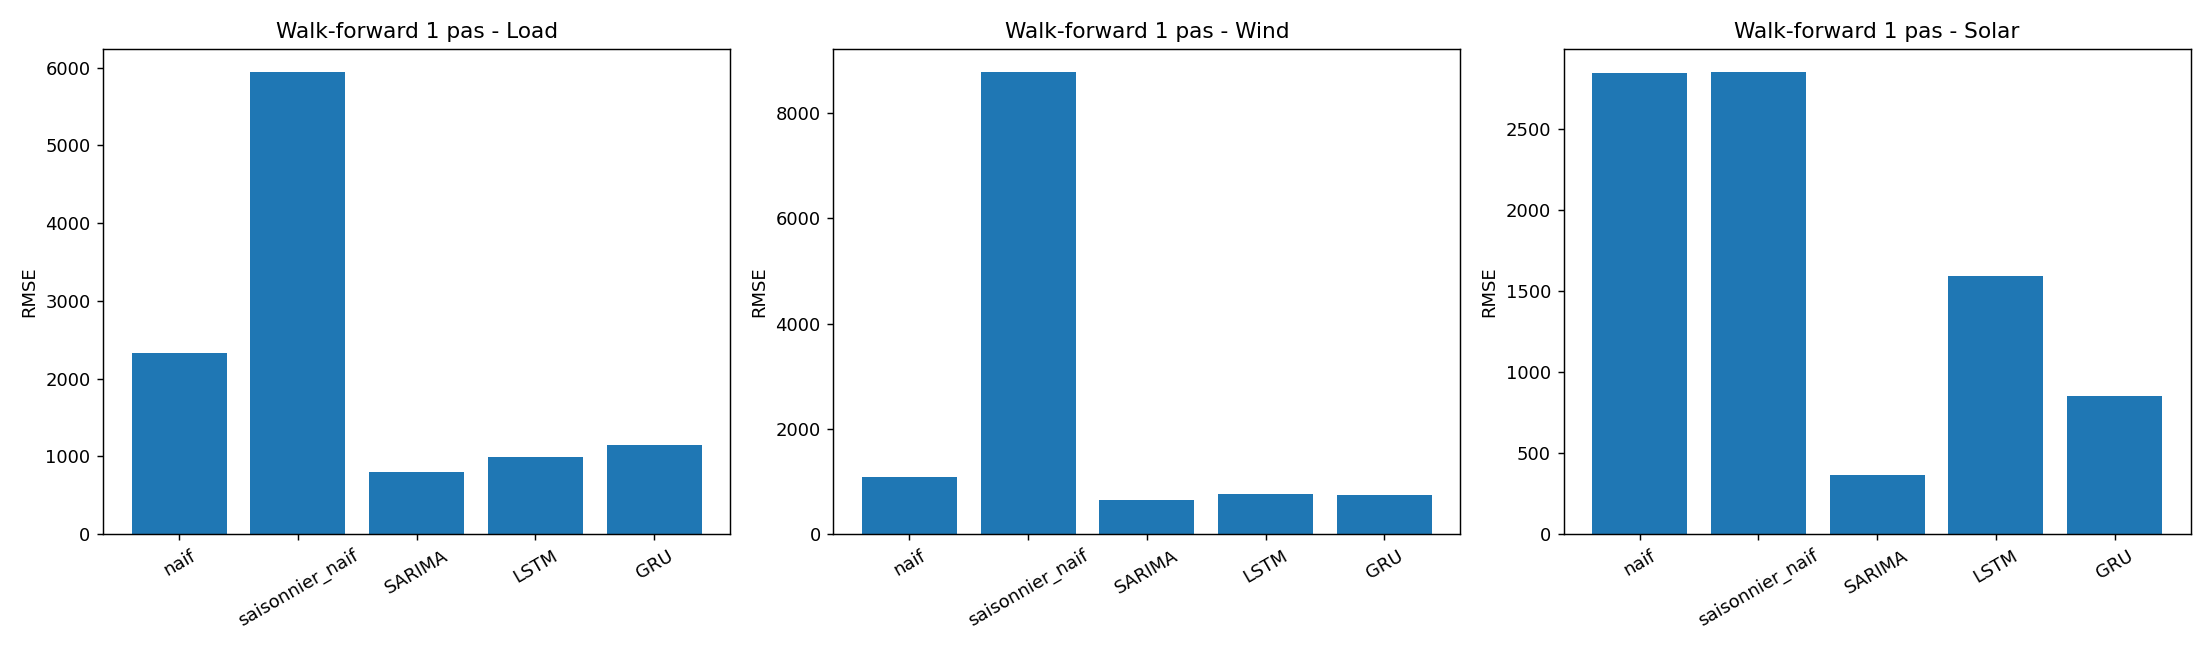
\includegraphics[width=0.95\textwidth]{py_evaluation_rmse.png}
\caption{Comparaison des RMSE par variable et par horizon.}
\label{fig:eval_rmse}
\end{figure}

\subsection{Walk-forward à un pas}
L'évaluation walk-forward à un pas confronte les baselines \emph{naïve} et
\emph{saisonnière-naïve} (\(24\)~h) au SARIMA retenu, au LSTM et au GRU, sur
les \(5\,040\)~h du test. Le tableau~\ref{tab:walkforward} montre que le
\textbf{SARIMA} obtient les meilleures métriques pour les trois séries
(\texttt{Load}\,: RMSE \(797{,}1\) contre \(998{,}3\) pour le LSTM ;
\texttt{Solar}\,: \(367{,}0\) contre \(856{,}0\) pour le GRU). Les réseaux
récurrents restent néanmoins nettement supérieurs aux modèles naïfs. Les
prévisions sont archivées dans \texttt{results/forecasts/py\_walkforward\_*.csv}.

\begin{table}[H]
\centering
\caption{Métriques walk-forward à un pas.
Source : \texttt{py\_walkforward\_metrics.csv}.}
\label{tab:walkforward}
\small
\begin{tabular}{llrrr}
\toprule
Variable & Modèle & MSE & RMSE & MAE \\
\midrule
\texttt{Load}  & naïf             & 5\,420\,103 & 2\,328{,}1 & 1\,807{,}0 \\
\texttt{Load}  & saisonnier naïf  & 35\,376\,448 & 5\,947{,}8 & 3\,889{,}6 \\
\texttt{Load}  & SARIMA           & 635\,357 & 797{,}1 & 590{,}3 \\
\texttt{Load}  & LSTM             & 996\,585 & 998{,}3 & 771{,}7 \\
\texttt{Load}  & GRU              & 1\,307\,527 & 1\,143{,}5 & 875{,}7 \\
\texttt{Wind}  & naïf             & 1\,187\,705 & 1\,089{,}8 & 782{,}6 \\
\texttt{Wind}  & saisonnier naïf  & 77\,192\,711 & 8\,785{,}9 & 6\,358{,}1 \\
\texttt{Wind}  & SARIMA           & 427\,719 & 654{,}0 & 452{,}9 \\
\texttt{Wind}  & LSTM             & 577\,189 & 759{,}7 & 552{,}9 \\
\texttt{Wind}  & GRU              & 544\,219 & 737{,}7 & 520{,}4 \\
\texttt{Solar} & naïf             & 8\,114\,702 & 2\,848{,}6 & 1\,889{,}3 \\
\texttt{Solar} & saisonnier naïf  & 8\,153\,433 & 2\,855{,}4 & 1\,417{,}7 \\
\texttt{Solar} & SARIMA           & 134\,710 & 367{,}0 & 245{,}0 \\
\texttt{Solar} & LSTM             & 2\,549\,469 & 1\,596{,}7 & 1\,344{,}4 \\
\texttt{Solar} & GRU              & 732\,792 & 856{,}0 & 659{,}0 \\
\bottomrule
\end{tabular}
\end{table}

\subsection{Test de Diebold--Mariano}
Le test de Diebold--Mariano est appliqué à \textbf{toutes les paires} de
modèles du walk-forward sur les erreurs quadratiques (un pas), avec
correction HLN et variance HAC (retard 1). Le tableau~\ref{tab:dm} en
présente les comparaisons clés. Toutes les statistiques sont hautement
significatives (\(p\)-valeurs \(<10^{-18}\) dans l'écrasante majorité des
cas) : sans ambiguïté, le \textbf{SARIMA est statistiquement meilleur} que
les naïfs, le LSTM et le GRU pour les trois séries. Entre réseaux, le
\textbf{LSTM} l'emporte sur \texttt{Load} et le \textbf{GRU} sur
\texttt{Wind} et \texttt{Solar}.

\begin{table}[H]
\centering
\caption{Test de Diebold--Mariano (extrait des paires du walk-forward).
Source : \texttt{py\_diebold\_mariano.csv}.}
\label{tab:dm}
\small
\begin{tabular}{llrrl}
\toprule
Variable & A vs B & DM stat & $p$-valeur & Conclusion \\
\midrule
\texttt{Load}  & naïf vs SARIMA            & $+38{,}62$ & $4{,}37\text{e-}286$ & SARIMA meilleur \\
\texttt{Load}  & saisonnier naïf vs SARIMA & $+34{,}60$ & $1{,}56\text{e-}235$ & SARIMA meilleur \\
\texttt{Load}  & SARIMA vs LSTM            & $-16{,}19$ & $1{,}65\text{e-}57$  & SARIMA meilleur \\
\texttt{Load}  & SARIMA vs GRU             & $-24{,}11$ & $1{,}25\text{e-}121$ & SARIMA meilleur \\
\texttt{Load}  & LSTM vs GRU               & $-12{,}07$ & $4{,}17\text{e-}33$  & LSTM meilleur \\
\texttt{Wind}  & naïf vs SARIMA            & $25{,}44$  & $2{,}01\text{e-}134$ & SARIMA meilleur \\
\texttt{Wind}  & saisonnier naïf vs SARIMA & $35{,}92$  & $9{,}97\text{e-}252$ & SARIMA meilleur \\
\texttt{Wind}  & SARIMA vs LSTM            & $-14{,}63$ & $1{,}69\text{e-}47$  & SARIMA meilleur \\
\texttt{Wind}  & SARIMA vs GRU             & $-11{,}26$ & $4{,}85\text{e-}29$  & SARIMA meilleur \\
\texttt{Wind}  & LSTM vs GRU               & $8{,}87$   & $1{,}03\text{e-}18$  & GRU meilleur \\
\texttt{Solar} & naïf vs SARIMA            & $44{,}27$  & $0{,}00$             & SARIMA meilleur \\
\texttt{Solar} & saisonnier naïf vs SARIMA & $21{,}60$  & $5{,}05\text{e-}99$  & SARIMA meilleur \\
\texttt{Solar} & SARIMA vs LSTM            & $-63{,}20$ & $0{,}00$             & SARIMA meilleur \\
\texttt{Solar} & SARIMA vs GRU             & $-31{,}18$ & $2{,}55\text{e-}195$ & SARIMA meilleur \\
\texttt{Solar} & LSTM vs GRU               & $39{,}75$  & $9{,}23\text{e-}301$ & GRU meilleur \\
\bottomrule
\end{tabular}
\end{table}

\paragraph{Nuance importante.}
Ce résultat concerne la prévision \textbf{à un pas} (walk-forward). Il met en
évidence la supériorité du SARIMA à un pas (filtre de Kalman mis à jour),
qui ne contredit pas l'avantage des modèles profonds sur les \emph{trajectoires
récursives} multi-pas (cf. tableau~\ref{tab:lstm}), ni l'explosion du MAPE
pour \texttt{Solar}. Le test DM entre SARIMA et LSTM sur les trajectoires
\(h>1\) constitue une piste d'approfondissement
(cf. section~\ref{sec:conclusion}).
